\documentclass{article}
\PassOptionsToPackage{numbers,sort&compress}{natbib}
\usepackage{neurips_2025}
\usepackage[utf8]{inputenc}
\usepackage[T1]{fontenc}
\usepackage{hyperref}
\usepackage{url}
\usepackage{booktabs}
\usepackage{amsfonts,amsmath}
\usepackage{microtype}
\usepackage{xcolor}
\usepackage{graphicx}
\newcommand{\todo}[1]{\textcolor{red}{[TODO: #1]}}
\newcommand{\absrel}{AbsRel}

\title{Where Does Equirectangular Distortion Really Hurt Panoramic Depth? \\
A Measurement Study and Inference-Time Corrections for Frozen Models}

\author{Aurindum Banerjee \\ IIT Jodhpur \\ \texttt{b23cs1006@iitj.ac.in} \And Harshita \\ \todo{surname, affiliation} \And Lokesh \\ \todo{surname, affiliation}}

\begin{document}
\maketitle

\begin{abstract}
Monocular depth models are applied to $360^\circ$ panoramas stored as equirectangular projections (ERP), whose rows are stretched by $1/\cos\phi$ towards the poles. The usual assumption is that this stretching explains the larger polar error. We test that assumption on four frozen models (MiDaS DPT-Hybrid, DAP, DA360, DA$^2$) and six datasets, using sweeps that move the \emph{same} content to different latitudes while keeping the ground truth fixed, with cluster-robust statistics and a rule for when an effect counts as measurable. We find that the projection itself explains little: rotating polar content to the equator does not help any model, DAP's large response to magnified polar content is a metric scale cue and disappears when the scale is re-fitted, and only DA360 shows a genuine, moderate sensitivity. Rotation-based inference ensembles help the older perspective-trained MiDaS (up to $+47\%$ polar error reduction on Structured3D) but hurt the metric foundation model DAP. What does hurt modern models are ordinary capture faults: a missing or blocked top/bottom, camera tilt, shake and JPEG compression. We catalogue ten such faults with physical causes, evaluate model-agnostic inference-time fixes for each, and combine the ones that help into a single correction step whose per-model choices are learned on held-out data and switched off when they would hurt. \todo{one sentence with the final held-out end-to-end numbers once the rerun with the fixed cap detector finishes}
\end{abstract}

\section{Introduction}
Panoramic depth estimation is moving from adapting perspective networks~\cite{rey2022360monodepth,wang2024depthanywhere} to dedicated panoramic foundation models~\cite{zhu2024panda,guo2025dac,lin2025dap,jiang2025da360}. ERP stretches content near the poles, so polar regions are the natural place to look for failures, and the natural fixes are to view the pole through a tangent-plane projection or to run the model on rotated copies of the panorama and fuse the results. Retraining is costly, so we ask what can be done at inference time, with the model frozen.

Our starting question is whether the polar error is a \emph{distortion} effect at all. A content effect (ceilings are bland, floors cluttered), a scale effect (a metric model sees smaller content as farther away) or an orientation effect (models expect up to be up) would all produce a latitude-dependent error without any projection problem. Our contributions are:
\begin{enumerate}
\item A measurement protocol that separates these causes (Section~\ref{sec:measure}) and its result on four models and six datasets: the polar deficit of current models is mostly not a projection effect.
\item An evaluation of two model-agnostic inference corrections, gradient-domain fusion and M\"obius test-time augmentation, with a compute-matched control. They help perspective-trained MiDaS and do not help panoramic foundation models.
\item A catalogue of ten realistic capture faults with inference-time mitigations, and a correction step that detects faults, selects the fix per model from held-out data, and leaves the model untouched when no fix helps.
\end{enumerate}

\section{Related work}
360MonoDepth~\cite{rey2022360monodepth} fuses depth from tangent perspective views; Depth Anywhere~\cite{wang2024depthanywhere} distils perspective models into panoramic ones; PanDA~\cite{zhu2024panda} adds M\"obius spatial augmentation for training; Depth Any Camera~\cite{guo2025dac} handles arbitrary camera models; DAP~\cite{lin2025dap} and DA360~\cite{jiang2025da360} are recent panoramic foundation models. \todo{short paragraph on distortion-aware convolutions and on test-time augmentation; add citations}

\section{Measuring the distortion effect}\label{sec:measure}
\paragraph{Sweeps.} For every frame the scene is rendered into the model at a series of latitudes and the error of the \emph{same pixels} is compared with the error in the pass where they sit closest to the equator. We use three modes: \emph{rotation} (the scene is tipped so polar content moves to the equator), \emph{dilation} (content is magnified as it would be near the poles but stays upright), and \emph{flip} (same latitude, upside down; the difference is an orientation penalty, not distortion). A real distortion effect must show in both rotation and dilation.
\paragraph{Estimators and onset.} The excess error $\Delta E(L)$ is computed with one global alignment of the prediction to the ground truth, and with the alignment re-fitted inside each latitude bin (the \emph{local} estimator, which removes scale effects). The onset latitude is the first of two consecutive 5$^\circ$ bins whose cluster-bootstrap lower confidence bound exceeds 10\% of the equator-seen error. Frames from one house, environment or street block form one cluster. Floors and ceilings (planar content) are separated from the rest.
\paragraph{Protocols.} Relative models (MiDaS, DA360) are scored after an affine fit; DA$^2$ after a scale fit; the metric model DAP is scored in raw metres, so scale is part of its error.

\section{Corrections}
\paragraph{Gradient-domain fusion and M\"obius test-time augmentation.} Method~1 re-estimates the polar cap from tangent views and merges them into the ERP prediction by solving a Poisson problem. Method~2 averages predictions from several M\"obius-rotated passes after re-anchoring each to the base pass. A \emph{yaw ensemble} with the same number of passes is the compute-matched control. \todo{one paragraph each with the equations; see project breakdown, Sections 4--5}
\paragraph{Capture faults.} Each fault in Table~\ref{tab:faults} has a physical cause, a simulator and one or more mitigations that return the prediction in the faulty frame, mapped back with a known transform. The correction step (i) re-levels with a known tilt, (ii) detects missing or occluded polar caps from the image (a uniform region whose edge is a constant latitude, tolerant to the $\pm1.4^\circ$ edge wobble seen on real Stanford2D3D captures), (iii) deblurs with a known kernel, and (iv) applies a fix only if the policy for that model and fault says so. The policy is learned from held-out datasets: a fix is kept when it lowers the median error by more than 2\% and improves at least 60\% of frames on the training sets, otherwise it is off. Stanford2D3D and NYC are never used to choose or tune anything.

\section{Experimental setup}
\paragraph{Models (all frozen).} MiDaS DPT-Hybrid (relative, perspective), DAP (metric, panoramic), DA360 (relative, panoramic), DA$^2$ (scale-only, panoramic).
\paragraph{Datasets.} Structured3D (rendered indoor), PanoX (rendered indoor and outdoor), Holo360D indoor and outdoor (real, LiDAR mesh; outdoor has only 3 clusters), and the external sets Stanford2D3D (real indoor; frames carry black caps above $65^\circ$) and NYC street panoramas (147 frames, 82 blocks, sky masked beyond 100\,m). Capture-fault studies use 40 frames per cell.

\section{Results}
\subsection{The polar deficit is mostly not a projection effect}
\begin{figure}[t]\centering
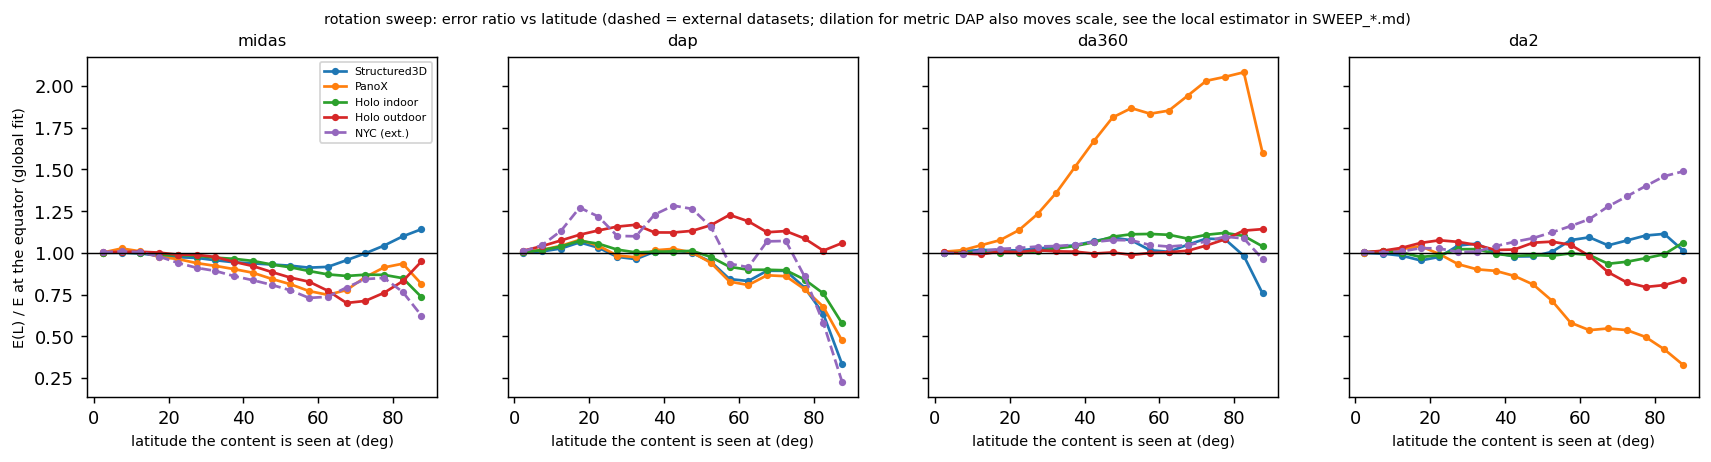
\includegraphics[width=\linewidth]{figs/fig_sweeps_rotation.png}\\[2pt]
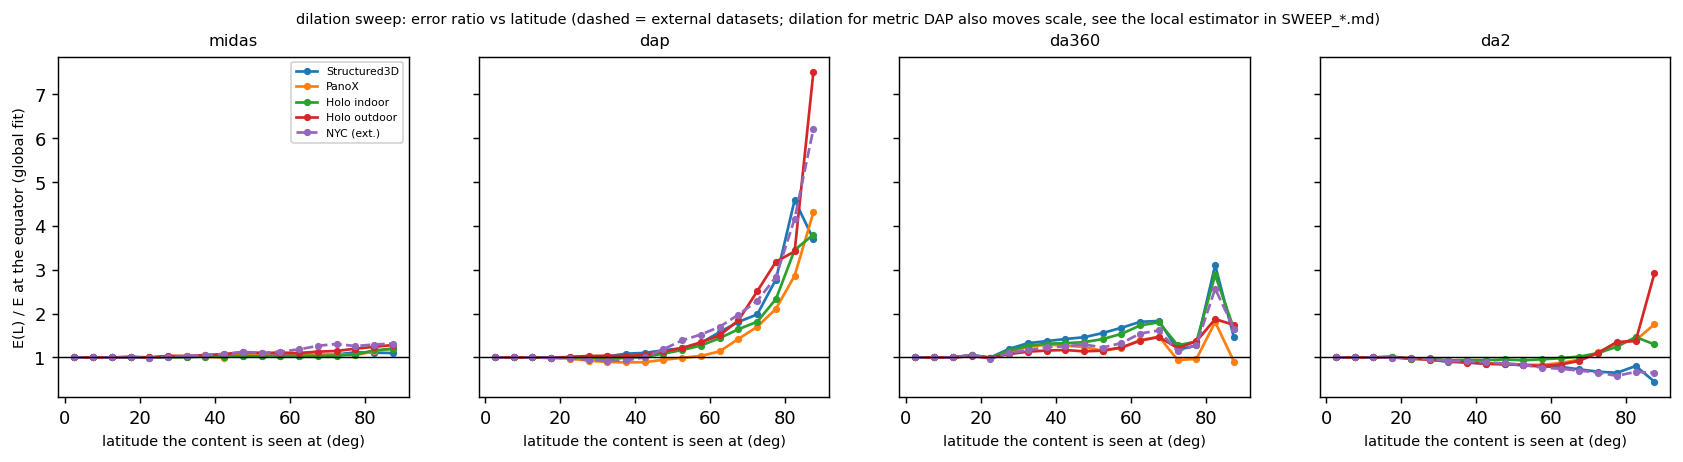
\includegraphics[width=\linewidth]{figs/fig_sweeps_dilation.png}
\caption{Error ratio versus the latitude at which the content is seen (global estimator). Top: rotation. Bottom: dilation. Dashed lines are external datasets. \todo{replace by the final figure once the NYC and Stanford sweeps are decided; add the local estimator panel}}\label{fig:sweeps}
\end{figure}
Rotation produces no onset for MiDaS, DAP or DA$^2$ on any core dataset, and only DA360 on PanoX (70$^\circ$). Dilation is different: on Structured3D DAP's global excess at 75--90$^\circ$ is $1.26$ (ratio $3.69$, onset $45^\circ$), but this is a scale cue. At $77.5^\circ$/$87.5^\circ$ the content is shrunk $2.5$--$7\times$ (log magnification $-0.90$ to $-1.97$), DAP reads smaller content as farther away, and the local estimator, which re-fits the scale, drops the excess to $0.013$ and $-0.14$. DA360's effect survives the local fit (local $\Delta E$ $0.04$--$0.14$ at the same bins, ratio up to $1.95$, onset $25^\circ$), a genuine but moderate sensitivity. MiDaS and DA$^2$ show essentially none (ratios $1.11$ and $0.64$ on Structured3D, no onset).

The orientation prior is real: upside-down content costs DAP $+0.07$ to $+0.18$ \absrel{} (ratio $3.18$ on Structured3D), DA360 ratio $1.85$ and DA$^2$ $1.48$ on Structured3D, and MiDaS $+0.15$ on PanoX. \todo{state the NYC sweep outcome: rotation onsets for DAP (15$^\circ$) and DA$^2$ (50$^\circ$) appear only under the global estimator and vanish under the local one; confirm from the SWEEP\_*\_nyc files and add Stanford (skipped: its real caps confound the sweeps)}

\subsection{Rotation ensembles help MiDaS, not the foundation models}
On Structured3D, three-pass M\"obius TTA reduces MiDaS's 75--90$^\circ$ error by $12.6\%$ (align-all) and $46.9\%$ (align-equatorial); five to seven passes give $22.6\%$ and $26.5\%$; PanoX gives $18.4\%$ with confidence intervals excluding zero. The yaw-only ensemble with the same compute stays within $\pm3\%$, so the gain is not averaging. For DAP the same ensemble worsens polar error indoors ($-32\%$ in raw metres on Structured3D). Holo outdoor shows gains for several models but rests on 3 clusters.

\subsection{Capture faults cost far more than the projection}
\begin{figure}[t]\centering
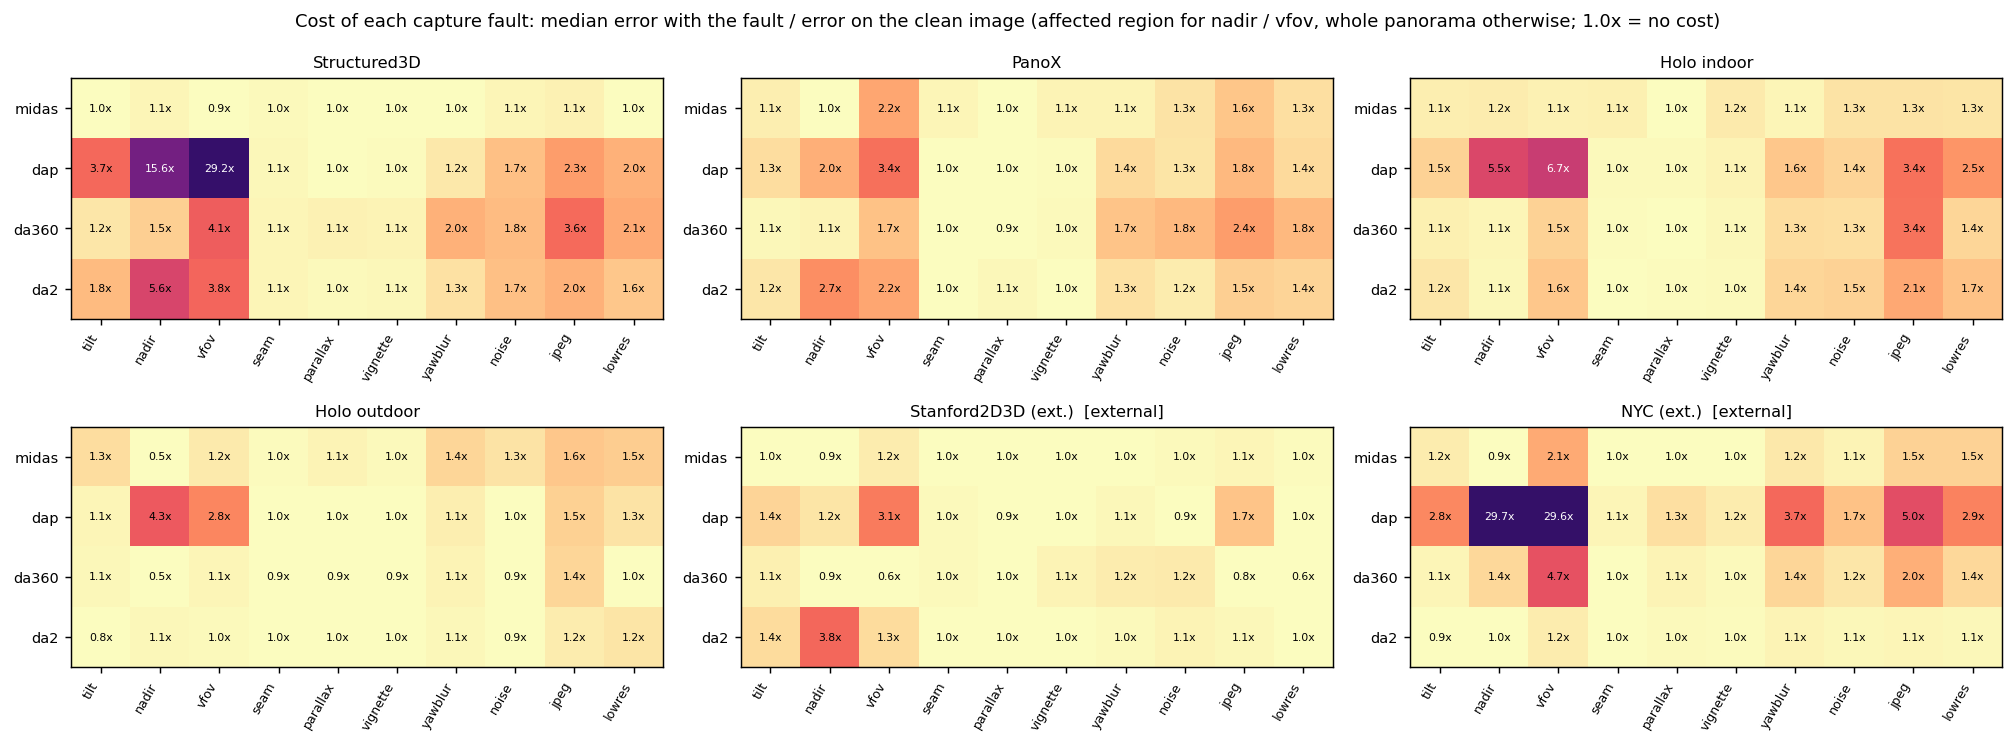
\includegraphics[width=\linewidth]{figs/fig_fault_cost.png}
\caption{Cost of each capture fault: median error with the fault divided by the error on the clean image, per model and dataset (affected region for nadir and field-of-view faults).}\label{fig:faultcost}
\end{figure}
Figure~\ref{fig:faultcost} shows that DAP is the most accurate model on clean images (\absrel{} $0.032$ on Structured3D against $0.221$ for MiDaS) and the most fragile under capture faults: removing the top and bottom of the panorama raises DAP's \absrel{} in the affected region from $0.026$ to $0.761$ on Structured3D, and a blocked bottom from $0.024$ to $0.372$. DAP is scored in raw metres and the other models after an alignment, which hides part of their errors, so absolute comparisons across models should be read with care.

\begin{table}[t]\centering\small
\caption{DAP, \absrel{} (affected region for caps, whole image for tilt), lower is better. Recovery is the median share of the damage undone over frames where the fault cost at least 5\%.}\label{tab:faults}
\begin{tabular}{lllrrrr}\toprule
Data & Fault & Fix & Clean & Faulty & Fixed & Recovery\\\midrule
S3 & tilt $12^\circ/8^\circ$ & re-level (IMU) & 0.032 & 0.120 & 0.038 & 96\%\\
PanoX & tilt & re-level (IMU) & 0.188 & 0.249 & 0.191 & 105\%\\
S3 & top/bottom missing & ERP inpaint & 0.026 & 0.761 & 0.286 & 64\%\\
PanoX & top/bottom missing & floor/ceiling plane fill & 0.187 & 0.643 & 0.342 & 73\%\\
PanoX & bottom blocked & plane fill & 0.111 & 0.222 & 0.143 & 85\%\\
\bottomrule\end{tabular}
\end{table}
Table~\ref{tab:faults} shows the strongest fixes. A fix that helps one model can hurt another: inpainting a blocked bottom makes DA360 worse on 85--92\% of frames, which is why the policy is learned per model. Denoising, bilateral smoothing, parallax seam inpainting and self-estimated tilt all harm clean or mildly faulty images and are excluded. Leave-one-dataset-out on the four core datasets selects a fix in 52 of 144 (model, fault, dataset) cells; 42 of those improve the median and 10 worsen it by at most 17\%, with a median change of $-8\%$ over applied cells. On clean images the correction step changes nothing.

\subsection{End to end and external validation}
\todo{Fill after the rerun with the fixed detector (STAGES="correct report"): held-out end-to-end table for the four models on the four core sets, then Stanford2D3D and NYC as external tests, with the share of frames improved and worsened. Do not quote earlier numbers: they used a cap detector that missed real Stanford caps at 512$\times$1024. Also pending: DA$^2$ on NYC re-scored with median alignment (its clean \absrel{} is 0.63, against 0.52 on Holo outdoor and 0.04 on S3), and cap fill before smoothing for JPEG plus blocked bottom.}

\section{Limitations}
Forty frames per fault cell and three clusters in Holo outdoor give wide intervals; faults are simulated, except the real caps of Stanford2D3D; tilt and shake fixes assume IMU or gyro data; DA$^2$'s least-squares scale fit may penalise outdoor scenes; and results for DAP are measured in raw metres while the others use alignment.

\section{Conclusion}
For current models the polar error is largely a content, scale and orientation effect, not a projection effect, so a universal polar correction has little to fix. Rotation ensembles remain useful for perspective-trained models. The practical gains come from handling ordinary capture faults, where a small learned policy of model-agnostic fixes recovers most of the damage for the strongest model, and leaves the others alone when it cannot help.

\begin{thebibliography}{9}
\bibitem{rey2022360monodepth} M.~Rey-Area, M.~Yuan, C.~Richardt. 360MonoDepth: High-resolution 360$^\circ$ monocular depth estimation. CVPR 2022 (arXiv:2111.15669).
\bibitem{wang2024depthanywhere} N.-H.~Wang, Y.-L.~Liu. Depth Anywhere: Enhancing 360 monocular depth estimation via perspective distillation and unlabeled data augmentation. 2024 (arXiv:2406.12849). \todo{check authors}
\bibitem{zhu2024panda} J.~Zhu, W.~Zhang, H.~Ai, H.~Bai, H.~Zhao, L.~Wang. PanDA: Towards panoramic depth anything with unlabeled panoramas and M\"obius spatial augmentation. 2024 (arXiv:2406.13378).
\bibitem{guo2025dac} Y.~Guo, S.~Garg, S.~M.~H.~Miangoleh, X.~Huang, L.~Ren. Depth Any Camera: Zero-shot metric depth estimation from any camera. 2025 (arXiv:2501.02464).
\bibitem{lin2025dap} X.~Lin, M.~Song, B.~Du, et al. Depth Any Panoramas: A foundation model for panoramic depth estimation. 2025 (arXiv:2512.16913). \todo{full author list}
\bibitem{jiang2025da360} H.~Jiang, Z.~Song, Z.~Lou, R.~Xu, M.~Tan, et al. Depth Anything in 360$^\circ$: Towards scale invariance in the wild. arXiv:2512.22819.
\end{thebibliography}
\end{document}
